% !TEX encoding = UTF-8
% !TEX TS-program = pdflatex
% !TEX root = ../tesi.tex
% !TEX spellcheck = it-IT

%**************************************************************
\chapter{Realizzazione}
\label{cap:realizzazione}
In questo capitolo vengono descritte le attività svolte durante lo sviluppo dell'applicazione e le principali difficoltà riscontrate.\\
Per lo sviluppo dell'applicazione sono state utilizzate, riadattandole, anche soluzioni sviluppate durante la fase di studio sui template, in particolare quelle relative al caricamento dei template e alla gestione delle librerie JQuery.\\
Durante questa fase il lavoro svolto è stato proposto al tutor aziendale in più riprese perché ne verificasse il comportamento e proponesse eventuali modifiche.
%**************************************************************

\section{Il caricamento dei template}
Il caricamento dei template consiste in tre fasi, che sono:
\begin{itemize}
	\item caricamento delle risorse;
	\item creazione istanza \textit{Ractive};
	\item rendering del template all'interno di un elemento HTML.
\end{itemize}
Per effettuare il caricamento delle risorse sono stati utilizzati due metodi differenti in base al tipo di file da caricare.\\
Il caricamento degli oggetti di tipo JSON, come i dati e l'elenco delle librerie JQuery del template, è stato effettuato tramite un metodo offerto dalla libreria JQuery, che permette di effettuare una \textit{GET HTTP request} per il caricamento specifico di oggetti JSON.\\
Il metodo in questione è \href{http://api.jquery.com/jquery.getjson/}{\texttt{jQuery.getJSON()}} che effettua una \textit{callback} ad un URL e ritorna l'oggetto desiderato.\\
Per effettuare il caricamento del template mustache invece, la comunità di Ractive offre un plug-in chiamato \texttt{ractive-load}\footnote{\url{https://github.com/ractivejs/ractive-load}} che aggiunge un metodo statico alla libreria e permette, tramite la  \textit{promise}\footnote{\url{http://www.ecma-international.org/ecma-262/6.0/\#sec-promise-objects}} \texttt{Ractive.load()} di effettuare il caricamento del file contenente la definizione del template utilizzando \textit{GET HTTP request}.
\newpage
\begin{lstlisting}[language=JavaScript, caption=Chiamate \textit{GET HTTP} per il caricamento delle risorse.]
// carico i dati del template
$.getJSON(dataUrl, function(dati) { // se il caricamento ha successo
	// carico il template tramite Ractive.load
	Ractive.load(tmlUrl).then( function(Template) {
		// creo l'oggetto ractive
		var ractive = new Template({
			el: tmlAnchor,
			data: dati
		});
	...

	});
})
.fail( function() { // errore caricamento, file non valido
	console.log('file non trovato o errore di caricamento!');
});
\end{lstlisting}
Le richieste vengono eseguite in modo asincrono, quindi solamente l'esito positivo della prima \textit{callback} permette l'esecuzione della chiamata a \texttt{Ractive.load()} e l'eventuale istanziazione dell'oggetto \textit{Ractive}.\\
Per quanto riguarda il caricamento di template contenenti plug-in JQuery, il metodo è identico, ma prima di caricare i dati ed il template devono essere caricate le librerie.\\
Il caricamento delle librerie viene effettuato tramite \texttt{JQuery.getJSON()} del file contenente la lista delle librerie e aggiungendo le URL di quest'ultime all'\texttt{header} dell'applicazione tramite la creazione di un tag \texttt{script} per ogni libreria individuata.\\
\begin{lstlisting}[language=JavaScript, caption=Codice per l'aggiunta delle librerie più esempio di JSON e risultato ottenuto.]
// carico le librerie del template
$.getJSON(libsUrl, function(libs) { // se il caricamento ha successo
	// aggiungo le librerie alla pagina HTML
	scriptControll.loadLibs(libs);

	// carico i dati del template
	$.getJSON(dataUrl, function(dati) { // se il caricamento ha successo
		...
		// istanziazione oggetto ractive
})
.fail( function() { // librerie non trovate o errore di caricamento
	console.log('file non trovato o errore di caricamento!');
///////////////////////////////////////////////////////////////////////
// esempio oggetto JSON contenente le URL delle librerie
{
	"libs": [
		"templates/jtml1/lib/actuate-animate.min.js",
		"templates/jtml1/lib/jquery.drawsvg.min.js"
	]
}
///////////////////////////////////////////////////////////////////////
// esempio di risultato prodotto nell'HTML
<head>
		...
	<!-- script aggiunti -->
	<script src="templates/jtml1/lib/actuate-animate.min.js"></script>
	<script src="templates/jtml1/lib/jquery.drawsvg.min.js"></script>
</head>

\end{lstlisting}
Per i template con plug-in JQuery il problema principale è quello che il template venga renderizzato prima del caricamento delle librerie, questo comporta il non riconoscimento delle funzioni che si riferiscono al plug-in rendendo il template incompleto.\\
Quindi il caricamento delle librerie viene eseguito sempre prima di caricare gli altri elementi del template.\\
Nonostante questa accortezza risulta impossibile verificare l'effettivo caricamento da parte del \textit{browser} delle librerie perché esso viene effettuato in modo asincrono.\\
Questo problema può essere risolto in maniera semplice con un \textit{reload} della pagina o come è stato fatto in un fork dell'applicazione tramite un \textit{preload} di tutte le librerie, che però risulta una soluzione molto onerosa e in certi casi non risolve il problema.

\subsection{Controllo delle librerie caricate}
Uno dei problemi che è sorto durante lo sviluppo in relazione al caricamento delle librerie per i template con plug-in JQuery, è quello di effettuare il caricamento di una o più librerie già caricate in precedenza.\\
Questo comporta la manipolazione inutile del \textit{DOM}, quindi una quantità maggiore di carico per il \textit{browser}.\\
Il problema è stato risolto effettuando un controllo tramite l'implementazione della funzione \texttt{confrontaScript()} che utilizza il metodo \texttt{document.scripts} per ricavare la lista delle librerie caricate dall'applicazione e tramite un confronto con essa decide se sia necessario aggiungere la nuova libreria o meno.\\
Questa funzione viene invocata dalla funzione \texttt{addLibraryFromUrl()} per ogni URL presente nel JSON, ogni qual volta venga caricato un template contenente plug-in.
\begin{lstlisting}[language= JavaScript, caption= Funzione che gestisce il caricamento di una libreria.]
confrontaScript(library) {
	var scriptArray = document.scripts; // array degli script caricati
	var trovato = false;
	for (var i = 0; i < scriptArray.length && !trovato; i++) {
		var scriptUrl = scriptArray[i].attributes.src.value;
		var scriptName = scriptUrl.slice( scriptUrl.lastIndexOf('/')+1, scriptUrl.length);
		if (scriptName === library) {
			trovato = true;
			//console.log('lo script '+library+' è già presente!');
		}
	}
	return trovato;
}

\end{lstlisting}

\section{Visualizzatore lista template}
Dopo aver sviluppato le funzioni per il caricamento dei template è iniziata la fase di realizzazione della sezione adibita alla visualizzazione della lista dei template disponibili.\\
Il problema che si è presentato prima di iniziare lo sviluppo è stato quello di scegliere quali elementi utilizzare per creare la lista.\\
La scelta più adeguata in questo caso sarebbe stata quella di caricare una lista di thumbnail (miniature) rappresentanti i vari template disponibili.\\
Questa decisione però, pur essendo la più efficiente, è stata scartata perché avrebbe richiesto la creazione di tutte le miniature e l'aggiornamento delle directory dei template.\\
Per questioni di tempo è stato deciso di caricare direttamente i template nella lista, visto che l'efficienza non era uno dei requisiti importanti per il tutor.\\
Dopo aver discusso il problema e definito il modo di procedere è iniziato lo sviluppo di questa sezione dell'applicazione.\\
La costruzione della lista viene effettuata creando i vari elementi che la compongono in modo sequenziale e inserendoli all'interno elemento HTML predisposto a contenerli.\\
Questa operazione viene effettuata dalle funzioni \texttt{createTemplateList()}, che tramite l'oggetto \hyperref[ttlObject]{\texttt{templatesToLoad}} si occupa di suddividere la lista fra le varie tipologie di template, e \texttt{loadTemplateList()}, che crea l'elemento \texttt{<li>} dedicato a contenere il template.\\
Il rendering viene effettuato all'interno dell'elemento \texttt{<li>} creato in precedenza utilizzando il suo id (creato in maniera univoca) come parametro di ancoraggio per l'oggetto \textit{Ractive} rappresentante il template.
\begin{lstlisting}[language=JavaScript, caption=Implementazione \texttt{loadTemplateList().}]
function loadTemplateList(type, num) {
	// per ogni tipo di template li carico tutti
	for (var i = 1; i < num+1; i++) {
		// creo list item ancora
		var listItem = "<li class='tml-list-item' ><div class='tml-list-item-div'><a class='tml-list-item-a' onclick='selectTml(this)' href='javascript:void(0)' id='"+type+i+"'></a></div></li>";
		// appendo l'elemento alla lista
		$('#tml-list').append(listItem);

		var anchor = '#'+type+i;
		// creo l'oggetto ractive col template relativo
		if (type === 'tml' || type === 'ctml') { // template senza jQuery
			var html = 'templates/'+type+i+'/'+type+i+'.html';
			var dati = 'templates/'+type+i+'/'+type+i+'.json';
			// carico il template
			tl.loadTemplateWithoutJQuery(html, dati, anchor);
		}
		else if (type === 'jtml' || type === 'jctml') { // template senza jQuery
			var html = 'templates/'+type+i+'/'+type+i+'.html';
			var dati = 'templates/'+type+i+'/'+type+i+'.json';
			var libs = 'templates/'+type+i+'/'+type+i+'_libs.json';
			// carico il template
			tl.loadTemplateWithJQueryPlugins(html, dati, libs, anchor);
		}

	}
}
\end{lstlisting}
\section{Visualizzatore template selezionato}
In questa fase di sviluppo è stata realizzata la \textit{view} dedicata alla visualizzazione del template selezionato.\\
Per effettua la visualizzazione è stato necessario:
\begin{itemize}
	\item individuare il template selezionato all'interno della lista;
	\item create un'istanza \textit{Ractive} che lo rappresenti;
	\item renderizzare il template all'interno della \textit{view}.
\end{itemize}
Per individuare il template selezionato è stato implementato l'evento \texttt{onclick} dei vari elementi appartenenti alla lista in modo che richiamino la funzione \texttt{selectTml()} passandogli il riferimento all'elemento che ha lanciato l'evento.\\
Dal riferimento è possibile risalire al nome del template da visualizzare e quindi creare un oggetto \textit{Ractive} che verrà renderizzato all'interno della \textit{view}.\\
Nel momento in cui viene visualizzato il template, viene richiamata la funzione che si occupa della costruzione del relativo editor, il cui sviluppo verrà descritto nella sezione seguente.
\begin{lstlisting}[language=HTML, caption=Chiamata di \texttt{selectTml()} all'evento \texttt{onclick} del list item.]
<li class='tml-list-item' >
	<div class='tml-list-item-div'>
		<a class='tml-list-item-a' onclick='selectTml(this)' href='javascript:void(0)' id='"+type+i+"'></a>
	</div>
</li>
\end{lstlisting}
Le modifiche ai dati sono visualizzate in tempo reale poiché la libreria \textit{Ractive.js} si occupa di effettuare l'update del render in maniera automatica.

\section{Editor per la manipolazione del template}
La realizzazione dell'editor per la modifica dei dati conclude la fase di sviluppo.\\
L'applicazione deve fornire un editor adeguato ad ogni possibile template, quindi risulta necessario individuare i dati modificabili del template e il loro tipo per poter fornire gli strumenti adeguati per la loro modifica.\\
Durante questa fase sono state individuate varie soluzioni per risolvere questo problema.\\
Una di queste consisteva nell'effettuare il parsing del \textit{DOM} del template, individuando il tipo del dato da modificare in base al \textit{tag} HTML che lo conteneva.\\
Questa soluzione è stata scartata perché troppo onerosa da implementare e perché certi dati all'interno del template potevano essere frutto di espressioni o di funzioni implementate nella logica del template, fatto non deducibile da un parsing del \textit{DOM}.\\
La soluzione individuata consiste nell'effettuare il parsing dell'oggetto JSON contenente i dati del template, questo offre la sicurezza sulla quantità di dati modificabili, ma fa sorgere un'altro problema.\\
Il problema riscontrato consiste nel non poter rilevare vari tipi tra quelli descritti nella sezione \textit{Analisi dei requisiti}, come, per esempio i tipi \texttt{colore}, \texttt{immagine}, \texttt{URL}, perché non presenti fra i tipi primitivi in un oggetto JSON.\\
\subsection{Creazione dell'editor}
La realizzazione dell'editor viene effettuata dalla funzione \texttt{creaTml()} che, in base al tipo di template, decide se creare un editor per template semplici o composti.\\
Per template composti è stata implementata la funzione \texttt{creaEditorFullJson()} che si occupa di creare una \textit{text-area} contenente l'oggetto JSON e ne permette la modifica direttamente da codice.\\
Lo sviluppo dell'editor per i template semplici, che viene effettuato dalla funzione \texttt{creaEditor()}, è stato più complesso perché ha richiesto l'individuazione del tipo di ogni dato presente nel JSON e la creazione del relativo strumento.\\
Per effettuare la creazione dei vari strumenti e per individuare i tipi di dato è stata sviluppata la funzione \texttt{parse()} che, in modo ricorsivo, effettua il parse dell'oggetto JSON individuando il tipo dei dati e costruendo per ognuno di essi il relativo strumento di input.\\
Il problema della rilevazione dei tipi non primitivi è stato risolto tramite il confronto dei dati di tipo \texttt{string} con espressioni regolari che rappresentano i seguenti tipi:
\begin{itemize}
	\item \textbf{colore}, rappresentato sia in formato \textit{rgb} che esadecimale;
	\item \textbf{URL}, rappresentato come url generica a risorse web non di tipo immagine;
	\item \textbf{mail}, rappresentato come indirizzo di posta elettronica;
	\item \textbf{immagine}, rappresentato come url a risorse di tipo immagine nei formati \textit{jpg, jpeg, png, gif} e \textit{svg}.
\end{itemize}
Nel caso in cui il tipo rilevato sia un immagine viene costruito un input di tipo \textit{input-file} che permette il caricamento di un immagine da file-system.\\
Mentre per il tipo \textbf{colore} è stato utilizzato il plug-in JQuery \href{http://jscolor.com/}{jscolor}, che permette di visualizzare il colore e propone un utile \textit{color-picker} per effettuarne la modifica.\\
\begin{figure}[htp]
	\centering
	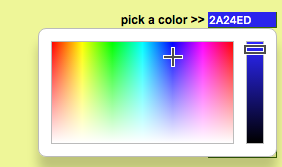
\includegraphics[scale=1]{../immagini/color_picker}
	\caption{Color-picker per la modifica dei tipi colore.}
\end{figure}
\newpage
Per la modifica degli altri tipi vengono utilizzati gli strumenti di input forniti dal linguaggio HTML senza ricorrere a librerie esterne.\\
In seguito viene proposto un estratto della funzione \texttt{parse()}.
\begin{lstlisting}[language=JavaScript, caption=Estratto della funzione \texttt{parse()}]
function parse(obj, el, index, regExpArray, path ){

	if (obj == null || obj == undefined) {
		return;
	}
	else {

	for (var k in obj) {

		if (typeof obj[k] === 'string') { // se è una stringa
			// controllo tramite regExp il tipo della stringa
			
			...

			if (pos === 0) { // è una e-mail
				label = "<label class='json-label'>"+k+": <input type='text' class='json-data-email edit' id='"+path+k+"' value='"+obj[k]+"' ></label><br>";
			}
			else if (pos === 1) { // è una URL
			
				if ( regExpArray[4].test(obj[k]) ) { // se true è un'immagine
					label = "<label class='json-label'>"+k+": <input type='file' class='json-data-img edit' id='"+path+k+"' ></label><br>";
				}
				else {
					label = "<label class='json-label'>"+k+": <input type='text' class='json-data-url edit' id='"+path+k+"' value='"+obj[k]+"' ></label><br>";
				}  
			}
			else if (pos === 2 || pos === 3) { // è un colore
				label =  "<label class='json-label'>"+k+": <span class='pick-color'>pick a color >> <input class='json-data-color jscolor edit' id='"+path+k+"' value='"+obj[k]+"'></span></label><br>";
			}
			else{ // è una normale stringa
				// costruzione input-text o text-area
				...
			}
		}

		else if (typeof obj[k] === 'number') { // se è una numero
			var label = "<label class='json-label'>"+k+": <input type='number' class='json-data-number edit' id='"+path+k+"' value='"+obj[k]+"' ></label><br>";
			$(el).append(label);
		
		}
		
		...
		
		// individuazione altri tipi e ricorsione per Array e Object
		
		...
	}
}
\end{lstlisting}

\subsection{Modifica dei dati}
La funzione \texttt{creaTml()} oltre ad occuparsi di creare l'editor giusto per ogni template, si occupa di aggiornare i dati in seguito a una modifica.\\
La modifica del model del template selezionato avviene tramite l'utilizzo del metodo \texttt{Ractive.set()}, offerto dalla libreria \textit{Ractive.js}.\\
Questo metodo modifica il model ed in seguito lancia l'evento \textit{update} che comporta il re-rendering del template nella pagina, permettendo la visualizzazione delle modifiche in tempo reale.\\

\subsection{Controllo degli input}
Prima di invocare la modifica di un dato viene effettuato un controllo sul dato inserito per verificarne la conformità con il tipo richiesto.\\
Per quanto riguarda i tipi non primitivi, citati in precedenza, vengono utilizzate le espressioni regolari per effettuare il controllo.\\
Nel caso in cui i dati inseriti non siano corretti viene visualizzato un messaggio di errore tramite un \textit{alert-box}.